\documentclass{minimal}
\usepackage[a4paper,margin=1cm,landscape]{geometry}
\usepackage{tikz}
\usetikzlibrary{positioning,shadows,arrows}

\begin{document}
\begin{center}
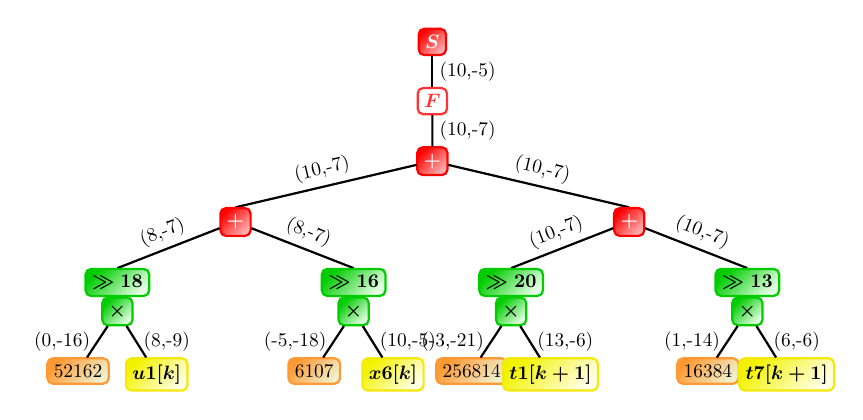
\begin{tikzpicture}[
	every node/.style={scale = 0.7},
	TreeNode/.style={rectangle,rounded corners=0.7mm, draw,
		text centered, font=\boldmath,anchor=north},
     form/.style={TreeNode,
		color=red!80, 
		fill=white, 
		text=red!80},
    form2/.style={TreeNode,
		color=blue!80, 
		fill=white, 
		text=blue!80},
    decM/.style={TreeNode,
		color=green!80!black,
		top color=green!80!black,
		bottom color=green!10,
		shading angle={45},
		text=black},
    adder/.style={TreeNode,
		color=red,
		top color=red,
		bottom color=red!30,
		shading angle={45},
        text=white},
    mult/.style={TreeNode,
		color=green!80!black,
		top color=green!80!black,
		bottom color=green!10,
		shading angle={45},
		text=black},
     cst/.style={TreeNode,
		color=orange!80, 
		top color=orange!80,
		bottom color=yellow!70!black!20,
		shading angle={45},
		text=black},
     var/.style={TreeNode,
		color=yellow!95!black,
		top color=yellow!95!black,
		bottom color=yellow!10,
		shading angle={45},
		text=black},
	 op/.style={TreeNode,
		color=green!30,
		top color=red!60,
		bottom color=green!30,
		shading angle={45},
		text=black},
    level distance=0.4cm, growth parent anchor=south, thick
]
\node (Sortie) [adder] {$S$}
child{[sibling distance=5.000000cm]
	node(DAdd_108) [form] {$F$}
	child{
		node(Add_108) [adder] {$+$}
	child{[sibling distance=3.000000cm]
		node(Add_107) [adder] {$+$}
		child{[sibling distance=1cm, level distance=0cm]
			node(DMultu1k lsb  7_M) [decM] {$\gg 18 $}
			child{[level distance=0.4cm]
				node(Multu1k lsb  7) [mult] {$\times$}
				child{
					node(Cst1) [cst] {52162}
				edge from parent node[left] {(0,-16)}
				}
				child{
					node(Var1) [var] {$u1[k]$}
				edge from parent node[right] {(8,-9)}
				}
			}
			edge from parent node[left,sloped,above] {(8,-7)}
		}
		child{[sibling distance=1cm, level distance=0cm]
			node(DMultx6k lsb  7_M) [decM] {$\gg 16 $}
			child{[level distance=0.4cm]
				node(Multx6k lsb  7) [mult] {$\times$}
				child{
					node(Cst2) [cst] {6107}
				edge from parent node[left] {(-5,-18)}
				}
				child{
					node(Var2) [var] {$x6[k]$}
				edge from parent node[right] {(10,-5)}
				}
			}
			edge from parent node[right,sloped,above] {(8,-7)}
		}
		edge from parent node[left,sloped,above] {(10,-7)}
	}
	child{[sibling distance=3.000000cm]
		node(Add_94) [adder] {$+$}
		child{[sibling distance=1cm, level distance=0cm]
			node(DMultt1k1 lsb  7_M) [decM] {$\gg 20 $}
			child{[level distance=0.4cm]
				node(Multt1k1 lsb  7) [mult] {$\times$}
				child{
					node(Cst0) [cst] {256814}
				edge from parent node[left] {(-3,-21)}
				}
				child{
					node(Var0) [var] {$t1[k+1]$}
				edge from parent node[right] {(13,-6)}
				}
			}
			edge from parent node[left,sloped,above] {(10,-7)}
		}
		child{[sibling distance=1cm, level distance=0cm]
			node(DMultt7k1 lsb  7_M) [decM] {$\gg 13 $}
			child{[level distance=0.4cm]
				node(Multt7k1 lsb  7) [mult] {$\times$}
				child{
					node(Cst3) [cst] {16384}
				edge from parent node[left] {(1,-14)}
				}
				child{
					node(Var3) [var] {$t7[k+1]$}
				edge from parent node[right] {(6,-6)}
				}
			}
			edge from parent node[right,sloped,above] {(10,-7)}
		}
		edge from parent node[right,sloped,above] {(10,-7)}
	}
		edge from parent node[right] {(10,-7)}	}
	edge from parent node[right] {(10,-5)}
}

;
        
\end{tikzpicture}
\end{center}
\end{document}